% Chapter 1

\chapter{Introduction} % Main chapter title
\label{Introduction} % For referencing the chapter elsewhere, use \ref{Chapter1} 
The following chapter starts with the motivation, why the autonomic management of service level agreements in cloud computing is a demanded capability (Section 1.1). Afterwards the limitations and shortcomings of the current cloud computing landscape, as well as the aim and objectives of this thesis are summarized (Section 1.2). Finally the structure is outlined (Section 1.3).

\section{Motivation}
Cloud computing has been one of the major trending topics of recent years in the Information Technology (IT) industry. A recent study about cloud adoption in Germany   \cite{BITKOM19} has shown that 73\% of the interviewed companies already use cloud solutions. In contrary to the older IT service delivery models, where all the services and resources where hosted locally, the idea behind cloud computing is to deliver computing resources or services on-demand over a network on an easy pay-per-use business model  \cite{NIST}. This paradigm change included almost all areas of the modern IT landscape, be it the storage and sharing of data for example with services like Dropbox  \cite{Dropbox}, Microsoft OneDrive  \cite{OneDrive} or Google Drive  \cite{GoogleDrive}, or complete computational environments like Amazon Web Services  \cite{AWS} or the Microsoft Azure Cloud Platform  \cite{Azure}. Nearly anything today is capable of being transferred to the cloud. As a result,  the investment costs for IT infrastructures or services can be lowered, since it is now obtained from a cloud provider and not bought or provided by the user himself. At the same time modern cloud providers posses an almost inexhaustible amount of computing resources pooled for their customers, so that nearly all requested amounts of resources can be provided within minutes.  Due to the lower upfront costs, rapid provisioning, elasticity and scalability, the adoption of cloud services is steadily increasing   \cite{IDC}. Thereby cloud computing nowadays for many companies has become a practical alternative to locally hosted resources and IT services. According to the analyst view of Gartner, the worldwide public cloud services market is projected to grow by 17.3\% in 2019 to total \$206.2B, up from \$175.8B   \cite{gart19}. This can be interpreted as a clear trend  towards the cloud business.

\begin{figure}[ht]
	\centering
	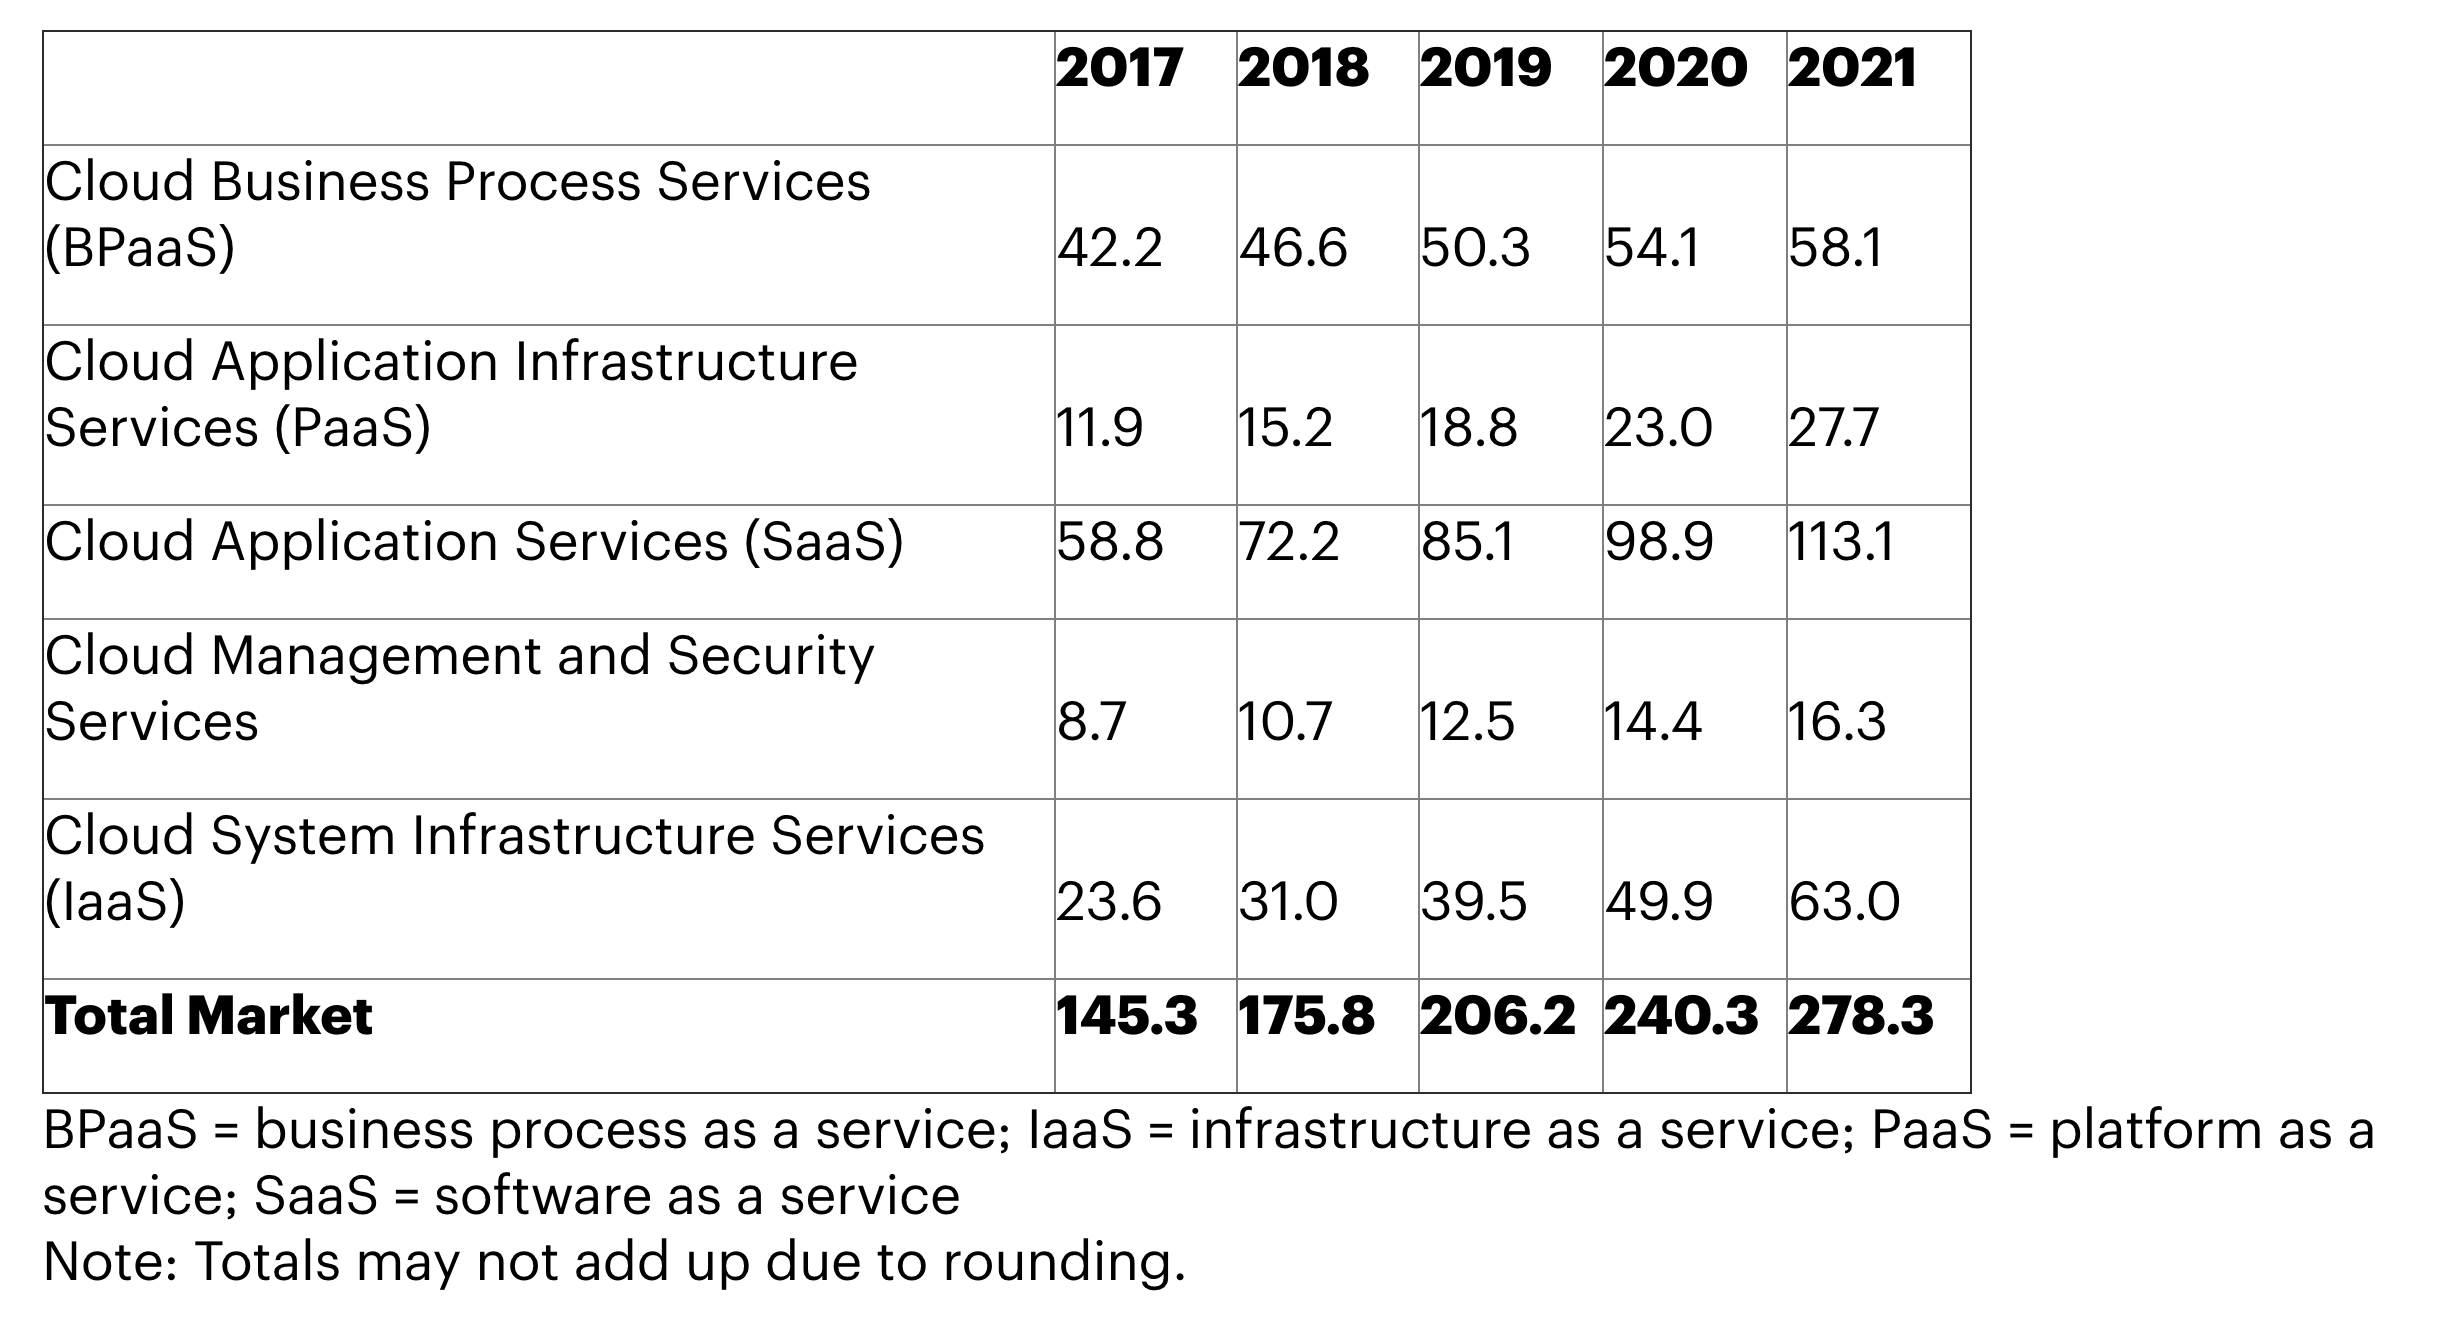
\includegraphics[width=0.7\linewidth]{chapters/chapter1/CloudRev}
	\caption{Worldwide Public Cloud Service Revenue Forecast (Billions of U.S. Dollars) Source: Gartner \cite{gart19}}
	\label{fig:cloudrev}
\end{figure}

However, in the current offered state of cloud computing, there are significant shortcomings in regard to guarantees and the quality of offered services. But such guarantees for bough services are desperately needed, especially by enterprises, to make could computing  effectively usable  \cite{DMTF2010} and reliable  \cite{JTC}. 
For this purpose so-called Service Level Agreements (SLA) are needed, which state the precise level of performance, as well as the manner and the scope of the service provided. This practice, which is widespread in the area of IT services, is currently of limited use for cloud computing, due to the fact that existing cloud environments offer only rudimentary support and handling of SLAs, if any. Therefore most providers do not offering any kind of SLA or just generic versions of standardized guarantees, such as availability or service and help desk. For example Amazon Web Services  \cite{AWS}, as one of the biggest players in cloud services only gives availability guarantees for their Elastic Compute Cloud (EC2)  \cite{EC2SLA}, which is simply stated as if the achieved monthly availability is below 99.95\% the the customer will be given back 10\% of the monthly fee in service credits. Additionally up to 30\% of the monthly fee will be credited if the availability falls below 99.0\%. There are no further performance or quality guarantees given so far. This means that without even having to pay credits back the EC2 cloud service can be down for 21.56 minutes every month plus maintenance. 

This is widespread for SLAs in the current cloud computing landscape  \cite{CloudSLAwhite}   \cite{Baset:2012:CSP:2331576.2331586} and does not offer any sufficient protection for the customer. In addition, practically unusable services, due to poor performance are not even taken into account. Arguably the compensation  through service credits is in not proportion to the expected actual financial damage that a company can suffer due to poor availability, which can render this whole SLA meaningless  \cite{meaning}. Cloud users should be given the opportunity to configure related services according to their needs and to obtain customized guarantees. So that users in need can protect particularly important services. This means that cloud providers must be able to provide the functionality of custom SLAs and be able to guarantee the corresponding quality of service parameters and demand a compensation. 



\section{Aim \& Research Questions}

In this section, the  aim and the research questions addressed in this thesis are presented.  Section 1.1 has shown the overview of the challenges motivating the research. Additionally, literature review on related work in the area of cloud computing guarantees, quality of service  and Service Level Agreements shows, that the following limitations exist: The classic SLA management approach is a rather static method, whereas due to the dynamic character of the cloud, the QoS attributes respectively service levels must be monitored and managed continuously \cite{Ludwig03WSLA}. Performance indicators \cite{5557978} and measurement methods for service level objectives in cloud computing have been studied inadequately \cite{Wieder2011}.
\\
The aim of the presented research has been to investigate the integration of SLAs into cloud computing environments to promote their reliability, transparency, trust and mitigate business concerns. Therefore cloud specific performance indicators, in dependence of cloud attributes such as, on-demand availability, elasticity of cloud resources and deployability were investigated. Following, an research of traditional SLA management and its ability to be integrated into the cloud has shown how there is need for changes. To address the identified problems  autonomic management of SLAs for cloud environments has been proposed.

Therefore, we concretely address the following research questions:
\begin{itemize} 
\item \textbf{How can Quality of Service Management and Service Level Agreements be  adapted and built-into Cloud Environments?}
For cloud computing, the quality and reliability of the services become an important aspect, as customers have no direct influence on the services. Due to the dynamic character and complex nature of the cloud environment, creating SLAs for the cloud can be very difficult. Therefore an adaptive autonomic architecture for cloud environments is needed.

\item \textbf{How can a Cloud provider manage and guarantee individual Cloud SLA objectives?}
Service requirements stated in Service Level Agreements need to be monitored and the corresponding resources need to be managed in order to guarantee them. In cloud systems, resources are being provided dynamically, which means the quality of a service can be directly
dependent on the provisioning mechanism. Hence  cloud computing services QoS monitoring, provisioning strategies, as well as detection and prediction of possible SLA violations must be proposed.

\item  \textbf{How can SLAs be enforced in the Cloud?}
The fulfilment of the agreed upon SLA objectives heavily depends on the manageability of the Cloud resources in the environment.
In order to efficiently provide theses resources an continuous autonomic control is necessary. Furthermore in case of SLA violations an superior management is needed.

\item  \textbf{How can we prevent and minimize SLA violations in the Cloud?}
SLA violations can happen especially due to varying demands and the up scaling delay of the infrastructure or economical limits. To minimize the number of SLA violations and to better guarantee the QoS, an behaviour, load and performance prediction based control model is needed. Additionally a violation management model is needed to optimise the outcome in cases where a violation could not be prevented.
\end{itemize} 




\section{Outline}
The remainder of this thesis is structured as follows. 

\textbf{Chapter 2} states background information to this study, starting with cloud computing its history,  definitions and a reference architecture to build a common knowledge base. Furthermore the foundations of Service Level Agreements, the process of SLA management as well as the guidelines on the content and preconditions will be given and the SLA life cycle will be introduced. Additionally the autonomic computing paradigm is introduced and discussed.\\

\textbf{Chapter 3} follows up on Service Level Agreements, by illustrating the current cloud computing SLA landscape and introducing cloud specific key performance indicators as basis for cloud service SLAs. Furthermore will the monitoring of cloud quality of service parameters and the controls and management will be elaborated.\\

\textbf{Chapter 4} presents the related work, which is divided into 6 categories: Infrastructure Measurements and Cloud Monitoring, SLA Description Languages, Performance Prediction, SLA Enforcement, Autonomic Computing and Scheduling Mechanisms. The related works of each section is analysed and distinctions to the contributions in this thesis are drawn.\\

\textbf{Chapter 5}  describes the presented approach for autonomic SLA management in cloud computing, starting wiht the introduction of the architecture and its modules. Subsequently the workflow from SLA creation to SLA monitoring and execution is illustrated to demonstrate the application of the autonomic SLA management.\\

\textbf{Chapter 6}- Implementation and Evaluations describes the developed prototype and its components. The Chapter follows the structure of the main research phases and presents the four consecutive development stages of the prototype:
\begin{itemize}
\item  Stage 1 - "ASLAMaaS Front-end" - The graphical user interface to build Cloud SLAs and exported in the machine readable A-SLO-A language.
 \item Stage 2 - KPI respectively SLA monitoring and enforcement with various management and prediction techniques.
 \item Stage 3 - Cloud Simulator integration for evaluation and proof of concept. 
 \item Stage 4 - Holistic SLA management based on provider prioritisation.
\end{itemize}
 Each section ends with a demonstration of its specific part of the development stage and a evaluation based on three scenarios is given in the end .\\

\textbf{Chapter 7} concludes the presented work and shows the  limitations of the proposed solutions. Afterwards the lessons learned during this study and possible future work arising from the research contributions of this thesis is described.\\

The Appendix shows the contributed research activities accompanying thesis with the published papers and reports. \\

Nomenclature
Within this thesis technical and legal terms are introduced at their first appearance. 
The terms cloud user, cloud consumer and cloud customer are used synonymously throughout this work.
